% Bản tiếng Việt đồng nhất claim và số liệu với bản tiếng Anh.
\documentclass[conference]{IEEEtran}
\IEEEoverridecommandlockouts
\usepackage{fontspec}
\setmainfont{Times New Roman}
\setsansfont{Arial}
\setmonofont{DejaVu Sans Mono}
\usepackage{graphicx}
\graphicspath{{figures/}{../../report/assets/}}
\usepackage{amsmath,amssymb}
\usepackage{booktabs}
\usepackage{array}
\usepackage{url}
\usepackage{balance}
\usepackage{microtype}

\title{Trade-off Precision--Recall Trong AEB Radar-Only, Camera-Gated Và Radar Emergency Fallback: Nghiên Cứu Tái Lập Trong CARLA}

\author{
\IEEEauthorblockN{Mai Việt Hoàng và Phạm Đức An}
\IEEEauthorblockA{\textit{Đại học Bách khoa Hà Nội}\\
Hà Nội, Việt Nam\\hoangmai04222@gmail.com}
}

\begin{document}
\maketitle

\begin{abstract}
Hard camera gate có thể chặn phanh nhầm do radar nhưng đồng thời phủ quyết vật
cản thật nằm ngoài không gian nhãn của detector. Bài báo định lượng trade-off này
và đánh giá radar emergency fallback trong pipeline AEB sensor-to-brake trên
CARLA 0.9.11. Điểm radar được lọc theo quỹ đạo, gom cụm, theo dõi và dùng tính
TTC/khoảng cách dừng; YOLO26n xác nhận lớp \emph{car}. Fallback chỉ cho phép
radar phanh khi track ổn định, đủ điểm, nằm giữa quỹ đạo và đồng thời có TTC,
stopping margin critical; quyết định được latch đến khi radar rời BRAKE. Chiến
dịch GPU khóa trước hold-out gồm 2.461 lượt chạy trong 639 phiên CARLA cô lập.
Trên core benchmark 525 lượt không tính synthetic fault, radar-only, hard gate
và fallback lần lượt đạt precision/recall 0,913/0,988, 1,000/0,965 và
1,000/0,988; fallback giảm collision của hard gate từ 25 xuống 15. Tuy nhiên,
frozen hold-out 70 lượt không cho thấy dominance: precision fallback giảm còn
0,600 do 20 false brakes trên synthetic ghosts 6--10 điểm; mọi chính sách đều
va chạm 15 lượt với ba physical props mới. Ablation, perturbation, camera-off và
CUDA timing chỉ ra cả điều kiện hữu ích lẫn failure mode còn lại. Kết quả ủng hộ
camera gate như cơ chế giảm false-positive và fallback như trade-off có điều
kiện, không phải giải pháp vật cản tổng quát hay chứng nhận an toàn.
\end{abstract}

\begin{IEEEkeywords}
phanh khẩn cấp tự động, camera--radar fusion, CARLA, phanh nhầm,
precision--recall, fault injection, hold-out
\end{IEEEkeywords}

\section{Giới thiệu}
AEB là vòng kín nhận thức--quyết định--chấp hành. Radar đo trực tiếp khoảng cách
và vận tốc xuyên tâm nhưng một return chưa chắc là vật cản thật trên đường ego.
Camera có thể loại mục tiêu radar không hợp lý, nhưng camera miss hoặc vật ngoài
nhãn không chứng minh đường trống. Vì vậy các tổng quan AEB xem nhận thức, quyết
định và điều khiển là chuỗi phụ thuộc \cite{yang2022aebreview}. Nhận dạng xe bằng
radar--vision và association cho AEB đã được nghiên cứu
\cite{kim2013vehicle,hsu2015noise}; bài báo không tuyên bố primitive fusion mới.

Mô phỏng cho phép lặp thí nghiệm gần va chạm
\cite{dosovitskiy2017carla,kang2019testing}, nhưng có hai bẫy: dùng actor truth
biến bài toán thành controller với trạng thái lý tưởng, và chỉ chạy lại scenario
đã dùng thiết kế rule có thể che biên thất bại. Nghiên cứu này dùng điểm radar và
frame RGB cho quyết định online, chỉ dùng actor truth để chấm; policy được khóa
trước hold-out và mọi case không đạt được giữ lại.

Bằng chứng trước cho thấy hard gate chặn 40/40 edge-prop false brakes nhưng bỏ
10/10 box/barrel giữa làn. Bản này đánh giá liệu radar emergency fallback có
phục hồi recall mà vẫn giữ precision hay không. Đóng góp gồm: (1) so sánh cố
định radar-only, hard gate và fallback; (2) ablation cùng one-factor sensitivity;
(3) perturbation, detector-disabled và frozen hold-out; (4) protocol GPU có
active-provider log, checkpoint và CARLA server mới cho mỗi named scenario. Kết
quả trung tâm gồm cả mặt âm: fallback kết hợp hai chỉ số core nhưng radar ghost
mạnh và prop mới ngăn claim dominance.

\section{Công trình liên quan và định vị}
Kim và Song kết hợp radar--vision để nhận dạng xe \cite{kim2013vehicle}; Hsu
\emph{và cs.} lọc nhiễu radar/camera cho lựa chọn mục tiêu AEB
\cite{hsu2015noise}. Bae \emph{và cs.} ước lượng xe gần nhất trong quỹ đạo bằng
LiDAR kênh thấp và camera trên xe thật \cite{bae2021cipv}. Zhang \emph{và cs.}
kết hợp nhận dạng mục tiêu đường cong, TTC, khoảng cách an toàn và phanh phân
tầng trong CarSim/Simulink \cite{zhang2023curved}. Vì vậy semantic verification,
path relevance và staged intervention không phải thành phần mới riêng lẻ.

CARLA đã được dùng để validation pipeline tự lái với scenario từ protocol
\cite{gomez2022carla}. Đóng góp của bài này là so sánh ba late-decision policies
có kiểm soát và hold-out bất lợi đã khóa, không phải detector/tracker mới. Hold-out
kiểm tra liệu rule phục hồi vật thể camera khó nhận có đồng thời nhận radar fault
mang cùng thuộc tính ở mức rule hay không. Cách đánh giá hướng falsification này
khác với chỉ demo scenario danh định.

\section{Hệ thống và ba chính sách}
\subsection{Ranh giới thông tin sensor-to-brake}
Hệ thống dùng Tesla Model 3 trên Town04, camera RGB và radar 100~m với sensor
tick 0,05~s. Radar CARLA là point-detection model, không phải chuỗi FMCW thô;
độ trung thực phụ thuộc cấp mô hình \cite{magosi2022radar}. Transform cảm biến
hiệu chuẩn phép chiếu, map height hỗ trợ loại ground. Logic phanh không truy vấn
actor ID, vận tốc/class actor hoặc ground-truth box; các giá trị này chỉ dùng
label và scoring.

Radar point được lọc theo range, height, road-ground và quỹ đạo độ cong không
đổi, sau đó gom cụm và ghép track. Track phải confirmed, không stale và liên
quan va chạm. Với khoảng cách $d$, vận tốc radar $v_r<0$:
\begin{equation}
 v_c=-v_r,\qquad \mathrm{TTC}=d/v_c.
\end{equation}
Với $v_t=\max(0,v_e+v_r)$:
\begin{equation}
 d_{\rm req}=\max\!\left(d_0,v_et_r+\frac{v_e^2}{2a_e}-
 \frac{v_t^2}{2a_t}+d_0\right),\quad m=d-d_{\rm req},
\end{equation}
trong đó $t_r=0,20$~s, $a_e=8$~m/s$^2$, $a_t=6$~m/s$^2$, $d_0=1$~m là tham số
mô phỏng. Staged PID đổi rủi ro thành lệnh phanh liên tục. Trong ablation riêng,
staged PID tránh thêm năm collision so với binary trên 330 system-limit runs.

YOLO26n được fine-tune một lớp \emph{car} bằng ảnh CARLA. Precision, recall,
$\mathrm{mAP}_{50}$ và $\mathrm{mAP}_{50:95}$ in-domain là 0,9919, 0,9642,
0,9940 và 0,9495; đây không phải metric an toàn AEB. Với target camera
$(X_c,Y_c,Z_c)$:
\begin{equation}
 u=f_xX_c/Z_c+c_x,\qquad v=f_yY_c/Z_c+c_y,\quad Z_c>0.
\end{equation}
Camera xác nhận nếu $(u,v)$ nằm trong YOLO car box; confirmation được giữ 0,35~s
theo simulation time.

\subsection{Ba chính sách phanh}
Radar-only truyền quyết định radar trực tiếp. Hard gate chỉ cho BRAKE khi camera
xác nhận hiện tại hoặc trong hold. Fallback dùng:
\begin{equation}
 B_f=B_r\land(C\lor H\lor E_r),
\end{equation}
trong đó $E_r$ yêu cầu track confirmed, không stale, age/hit streak $\geq3$, ít
nhất 6 điểm, confidence $\geq0,70$, path offset $\leq0,65$~m,
TTC $\leq1,10$~s và $m\leq-2,0$~m. TTC và margin phải cùng critical. Fallback
được latch đến khi radar rời BRAKE. Không dùng actor type/scenario label. Rule
này chỉ giới hạn override, không chứng minh track radar là vật thật.

\begin{table}[t]
\caption{Cấu hình emergency fallback đã khóa.}
\centering\footnotesize
\begin{tabular}{lr}
\toprule Điều kiện & Giá trị\\ \midrule
Track age / hit streak & $\geq3/3$ frame\\
Cluster points / confidence & $\geq6/0,70$\\
Path offset & $\leq0,65$ m\\
TTC / stopping margin & $\leq1,10$ s / $\leq-2,0$ m\\
Risk / release & TTC AND margin / latch\\
\bottomrule
\end{tabular}
\end{table}

\section{Protocol khóa trước hold-out}
Simulator chạy synchronous fixed-step 0,05~s với physics control. Policy v1 và
protocol được tag trước hold-out. Hard gate/fallback dùng cùng ONNX, input 640,
cadence 0,15~s simulation time và bắt buộc \texttt{CUDAExecutionProvider}; CPU
fallback hoặc inference error là hard stop. Master runner checkpoint từng run,
chạy repeat của một named scenario, dừng CARLA rồi khởi động Town04 mới. FAIL
thuật toán không dừng campaign.

2.461 lượt gồm 22 smoke, 324 development ablation/sensitivity, 1.665 core, 180
perturbation, 60 detector-disabled và 210 hold-out. Core có full66 CCRm/CCRb/
cut-in, regression hỗn hợp, 40 edge props, 10 box/barrel trung tâm và 30
synthetic faults bốn điểm có nhãn. Injection không đại diện ghost tự nhiên của
CARLA.

Hai mươi perturbations thay speed $\pm2$~km/h, gap $\pm1$~m, cut-in start
$\pm0,1$~s và box offset $\pm0,15$~m. Camera-off mô phỏng không có detection.
Frozen hold-out dùng shopping cart/bench/traffic warning, bốn vehicle appearances,
hai edge props và năm persistent ghosts 6--10 điểm. Không tuning v1 sau hold-out.

Nhãn dương nghĩa là cần phanh; prediction dương là đã kích hoạt phanh. Collision
và full PASS được báo riêng vì phanh TP vẫn có thể quá muộn. Precision/recall phụ
thuộc thành phần suite có chủ đích, không phải prevalence giao thông. Wilson CI
mô tả run-level; named-scenario consistency được kiểm tra riêng. Repeat không
được coi là encounter độc lập.

\section{Kết quả}
\subsection{Trade-off trên core}
Bảng~\ref{tab:main} loại synthetic faults khỏi ma trận chính. Radar-only recall
cao hơn hard gate nhưng có 40 edge-prop FP. Hard gate không FP nhưng bỏ mười
non-vehicle trung tâm và năm late cut-out. Fallback phục hồi mười lượt trung tâm
và vẫn không có core FP. Collision bằng radar-only (15) và thấp hơn hard gate
(25). Wilson CI 95\% của radar precision là 0,884--0,936; radar/fallback recall
0,973--0,995; hard recall 0,943--0,979; precision zero-FP 0,991--1,000. Khi cộng
30 synthetic faults yếu, radar precision giảm 0,857; hai camera policy chặn
30/30.

\begin{table}[t]
\caption{Core không tính synthetic fault (525 lượt/chính sách).}
\label{tab:main}
\centering
\footnotesize
\setlength{\tabcolsep}{3pt}
\begin{tabular}{lrrrrrrr}
\toprule
Chính sách & TP & FP & TN & FN & Prec. & Rec. & Coll.\\
\midrule
Radar-only & 420 & 40 & 60 & 5 & .913 & .988 & 15\\
Hard gate & 410 & 0 & 100 & 15 & 1.000 & .965 & 25\\
Fallback & 420 & 0 & 100 & 5 & 1.000 & .988 & 15\\
\bottomrule
\end{tabular}
\end{table}

Trên 555 core runs, fallback cải thiện 70 outcome so với radar-only, 10 so với
hard gate và không hồi quy. Đây chỉ là kết luận within-core; hold-out đảo chiều
so sánh với hard gate. Hình stress-suite cho thấy radar đạt central props nhưng
phanh ở mọi edge prop/fault, hard gate có kết quả ngược ở central props, còn
fallback đạt cả ba core stress families.

\begin{figure}[t]
\centering
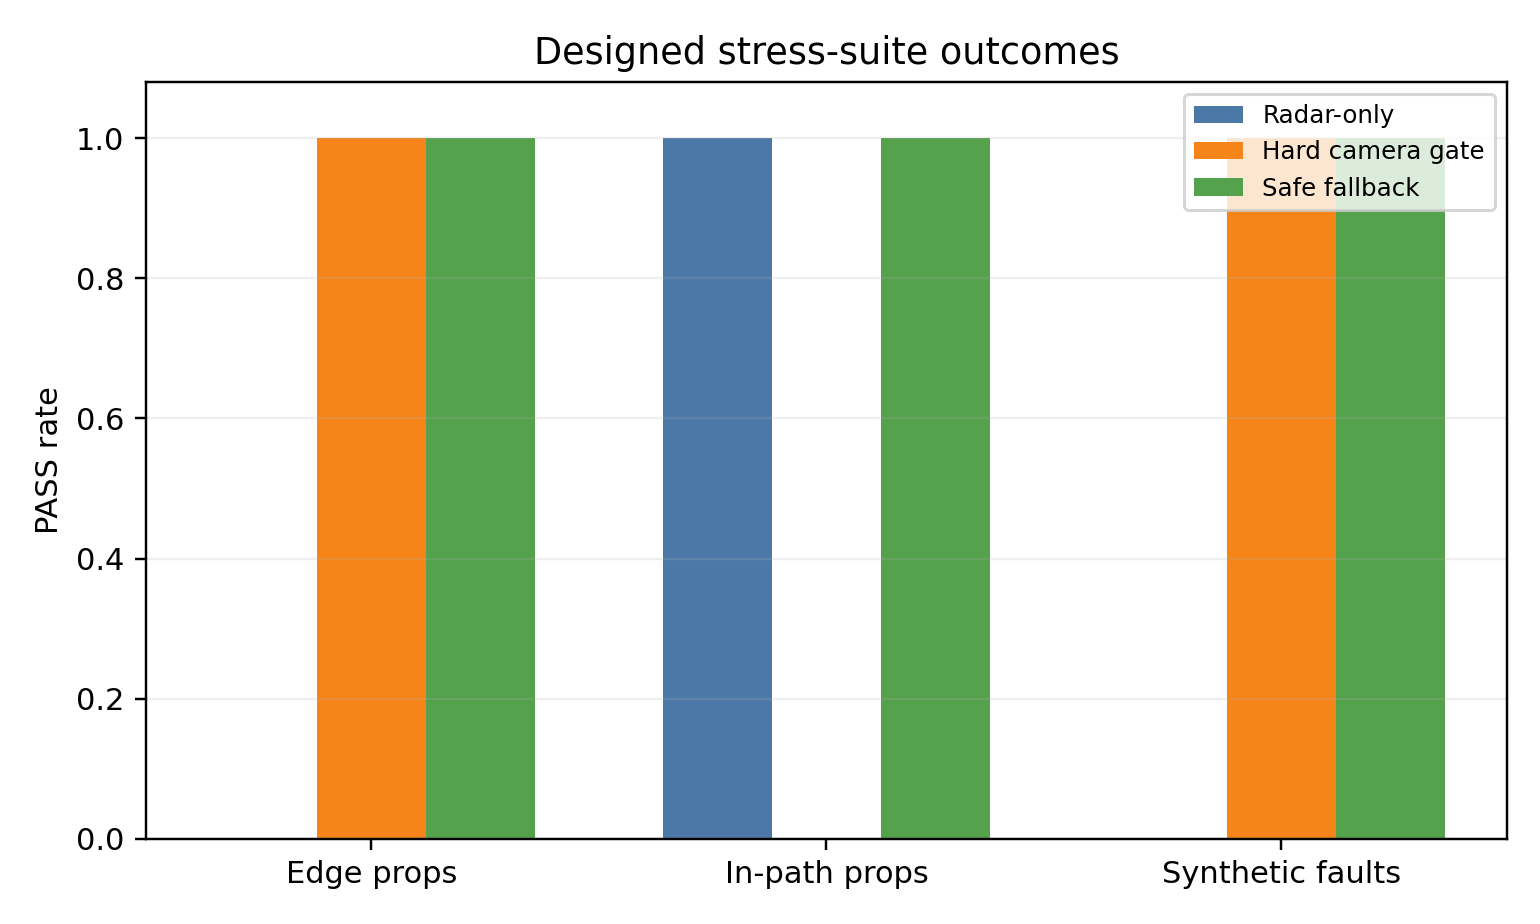
\includegraphics[width=0.98\columnwidth]{stress_suite_pass_rates.png}
\caption{Core stress-suite PASS rate; tỷ lệ class có chủ đích.}
\end{figure}

\begin{figure*}[t]
\centering
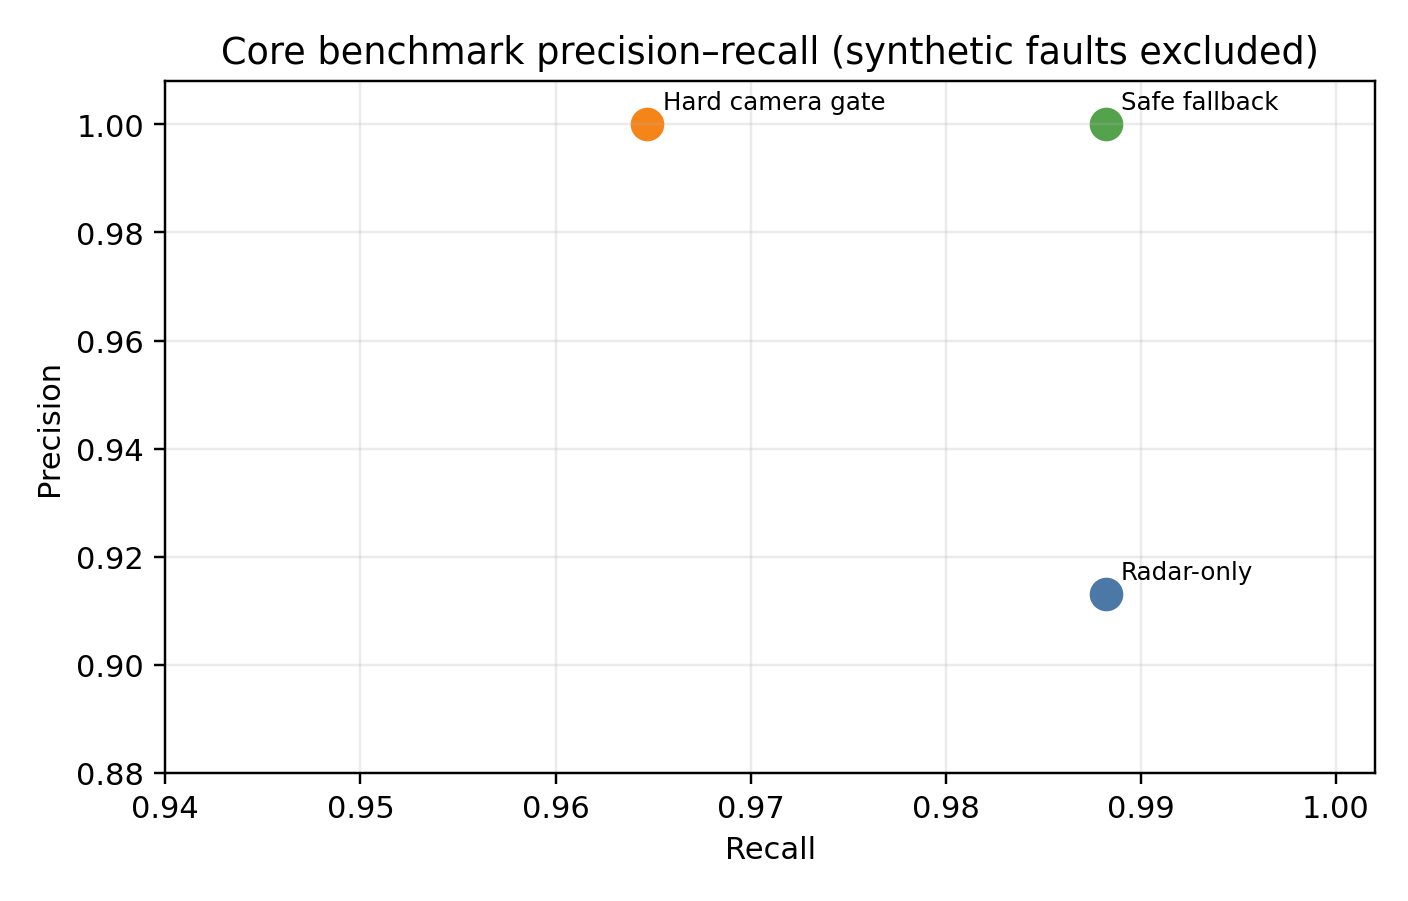
\includegraphics[width=0.47\textwidth]{core_precision_recall.png}\hfill
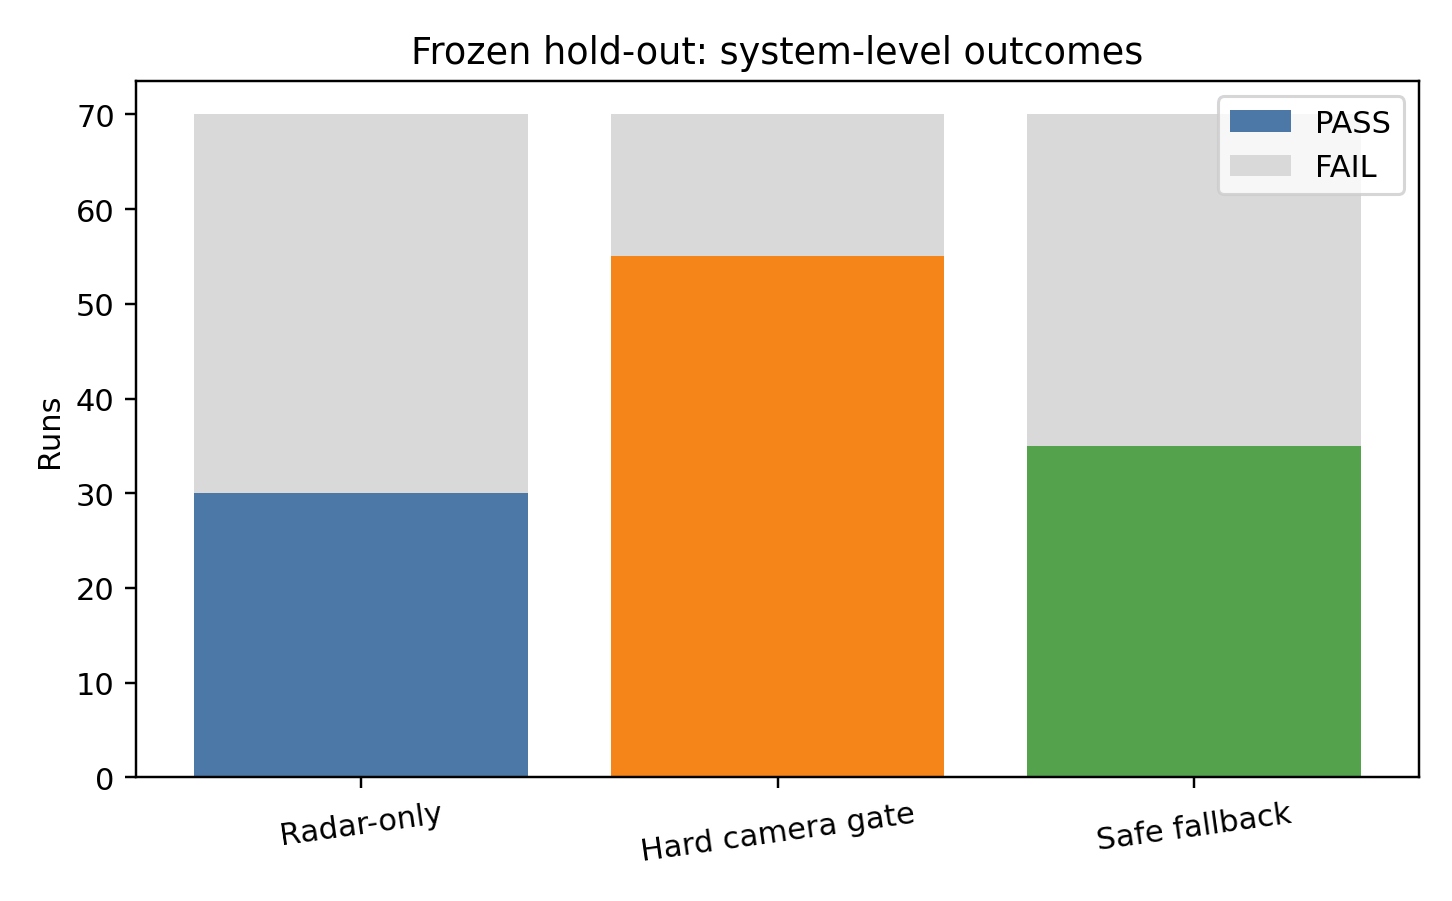
\includegraphics[width=0.47\textwidth]{holdout_pass_fail.png}
\caption{Trái: core precision--recall không tính synthetic fault. Phải:
PASS/FAIL hệ thống trên frozen hold-out. Tỷ lệ class do người thiết kế chọn.}
\label{fig:tradeoff}
\end{figure*}

\subsection{Ablation, sensitivity và degradation}
Ablation 12 scenario ×2: full fallback đạt 24/24. Hard gate và no-latch cùng
fail bốn central box/barrel; bỏ central-path gây sáu edge-prop false brakes; bỏ
point threshold gây bốn synthetic false brakes yếu. Bỏ stability/confidence
hoặc đổi TTC-AND-margin thành OR không đổi subset, nên chưa chứng minh tính cần
thiết độc lập của hai rule đó.

Sensitivity sáu scenario ×2: nominal 12/12. Giảm minimum points 6 xuống 4 gây
hai synthetic FP; tăng stability 3 lên 4 frame hoặc siết TTC 1,10 xuống 0,90~s
bỏ central box hai lần. Các biến thể path, margin, confidence và TTC permissive
không đổi subset. Đây là local trade-off, không phải tối ưu threshold.

\begin{table}[t]
\caption{Robustness và frozen hold-out.}
\label{tab:extended}
\centering
\scriptsize
\setlength{\tabcolsep}{3pt}
\begin{tabular}{llrrrrrr}
\toprule
Suite & Policy & Pass/N & TP & FP & TN & FN & Coll.\\
\midrule
Perturb. & Radar & 57/60 & 60 & 0 & 0 & 0 & 3\\
 & Hard & 45/60 & 45 & 0 & 0 & 15 & 15\\
 & Fallback & 54/60 & 60 & 0 & 0 & 0 & 6\\
\midrule
Camera off & Hard & 12/30 & 0 & 0 & 12 & 18 & 18\\
 & Fallback & 24/30 & 18 & 0 & 12 & 0 & 6\\
\midrule
Hold-out & Radar & 30/70 & 30 & 25 & 10 & 5 & 15\\
 & Hard & 55/70 & 25 & 0 & 35 & 10 & 15\\
 & Fallback & 35/70 & 30 & 20 & 15 & 5 & 15\\
\bottomrule
\end{tabular}
\end{table}

Trong perturbation, hard gate bỏ toàn bộ năm box; fallback phục hồi ba nhưng còn
collision ở gap 19/21~m dù nominal 20~m đạt. Radar-only cũng collision ở 19~m.
Đây là ảnh hưởng không đơn điệu của return geometry, thời điểm confirm và margin.
Khi camera off, fallback phanh ở 18/18 positive nhưng vẫn collision sáu lượt
stationary/braking lead do trigger muộn. Brake recall không đồng nghĩa safe stop.

\subsection{Frozen hold-out và CUDA timing}
Hold-out là bằng chứng không dominance. Mọi policy collision 15 lượt ở ba props
mới. Shopping cart chỉ tạo tối đa hai path candidates và không có target
confirmed; bench/warning trigger quá muộn. Fallback phản ứng với bốn ghosts
central/offset 0,50~m, gây 20 FP và chỉ chặn ghost offset 0,75~m. Precision/recall
hold-out là 0,600/0,857, so với hard gate 1,000/0,714. Paired system status:
hard-only PASS 20, fallback-only PASS 0, cùng PASS 35 và cùng FAIL 15. Fallback
phục hồi một số brake label nhưng không giải quyết unknown-obstacle detection.

Campaign ghi 474 CUDA sessions, 74.928 inference và 0 lỗi. Session-median
p50/p95 là 9,95/11,53~ms, weighted mean 11,56~ms. Mỗi process có một cold start
trên 150~ms; maximum 276,10~ms. Số liệu chứng minh steady-state throughput trên
GPU thử nghiệm và công bố startup cost; synchronous simulation chờ processing
nên không chứng minh deadline ECU.

\subsection{Phân rã failure mechanism và traceability}
Physical hold-out không phải một camera-gate failure đồng nhất. Shopping cart
chỉ có tối đa hai path candidates, không track confirmed nên không policy nào
phanh. Bench có track: radar-only phanh ở gap 12,62~m, fallback đợi emergency
đến 4,30~m, hard gate không phanh; tất cả collision. Traffic warning làm hard
gate phanh ở 21,87~m, cho thấy apparent camera confirmation, nhưng vẫn collision.
Ba mechanism là missing track, late qualification và collision/dynamics.

Ghost sáu điểm tạo một confirmed cluster và làm radar/fallback phanh ở 0,15~s,
trong khi hard gate chặn. Ghost tám/mười điểm tương tự; tại offset 0,75~m,
fallback chặn bằng threshold 0,65~m còn radar vẫn phanh. Precision loss vì vậy
là hệ quả trực tiếp của fallback evidence.

Mỗi child run lưu commit, seed, model/config SHA-256, phiên bản CARLA, fixed step,
active provider và gate reason từng tick. Archive có CSV/JSON, config snapshot,
manifest và SHA-256. Run-level Wilson interval không tạo independence; mọi named
condition hold-out/perturbation đều nhất quán all-PASS hoặc all-FAIL. Paired
hard/fallback core là 525 cùng PASS, 10 fallback-only và 20 cùng FAIL; hold-out
là 35 cùng PASS, 0 fallback-only, 20 hard-only và 15 cùng FAIL.

\section{Thảo luận và hạn chế}
\subsection{Hàm ý thiết kế}
Ba policy tương ứng error cost khác nhau, không phải xếp hạng tuyệt đối.
Radar-only là upper bound chẩn đoán recall nhưng phanh với mọi edge prop/fault.
Hard gate bảo thủ nhất với radar chưa xác nhận và có hold-out PASS cao nhất,
nhưng car-only semantics giới hạn non-vehicle recall. Fallback dịch về radar
recall và chỉ phù hợp nếu ODD chấp nhận failure mode high-support ghost.

Point count, confidence, persistence, path offset, TTC và margin đều là thuộc
tính của cùng track estimate; không thuộc tính nào độc lập chứng minh vật thể tồn
tại. Tăng threshold chặn fault yếu nhưng tiêu thụ stopping distance. Cần nguồn
bằng chứng mới như free-space, obstacle semantics rộng hơn, occupancy hoặc
multi-sensor existence probability thay vì tiếp tục chỉ tuning rule.

\subsection{Biên hiệu lực}
Evidence hỗ trợ kết luận hẹp hơn “fusion tốt hơn”. Camera gate giảm FP khi label
space bao phủ hazard. Fallback có thể phục hồi object ngoài nhãn, nhưng rule chấp
nhận stable/central/high-support track cũng dễ nhận stable/central/high-support
ghost. Tăng quality/risk threshold lại làm chậm hoặc bỏ vật thật, đúng như
sensitivity và camera-off thể hiện.

External validity bị giới hạn bởi một map/ego, ảnh thuận lợi, detector một lớp và
point-level radar. Synthetic ghost là fault model, không phải distribution
multipath đo được. Hold-out có thêm diversity nhưng nhỏ và cân bằng có chủ đích.
Không có HIL, actuator/communication delay, friction sweep, sensor data thật hay
xe thử nghiệm. CCR chỉ lấy cảm hứng, không tái tạo đầy đủ hoặc chứng nhận Euro
NCAP \cite{euroncap_aeb}. Hướng tiếp theo là uncertainty-aware tracking,
free-space/multi-class visual evidence, degradation theo thời gian, dữ liệu radar
camera ghi thật và objective impact-speed/stopping-margin trước khi tăng repeat.

\section{Kết luận}
Radar emergency fallback kết hợp hard-gate precision và radar-only recall trên
core benchmark, nhưng frozen hold-out chứng minh kết hợp này không tổng quát.
Radar ghost mạnh đánh đổi precision lấy recall; một số vật cản mới không được
track đủ sớm bởi mọi policy. Kết quả chính là bản đồ trade-off/failure tái lập:
camera gate chặn false brake, fallback phục hồi obstacle recall có điều kiện,
không phương án nào là giải pháp an toàn tổng quát. Mọi claim chỉ thuộc
synchronous CARLA, không phải NCAP, functional safety, triển khai real-time hay
kiểm định xe thật.

\balance
\bibliographystyle{IEEEtran}
\bibliography{references}
\end{document}
